\documentclass[letterpaper]{article}
\usepackage{inconsolata}
\usepackage[T1]{fontenc}
\usepackage[margin=1in]{geometry}
\usepackage[utf8]{inputenc}
\usepackage{hyperref}
\usepackage{soul}
\usepackage{fancyhdr, lastpage}
\usepackage{graphicx}
\pagestyle{fancy}
\fancyhf{}
\usepackage{minted}
\usemintedstyle{pastie}

\newcommand{\spacer}{\vspace{5mm}\hrule\vspace{5mm}}

\makeatletter
\renewcommand{\@maketitle}{
  \begin{center}%
    {\LARGE \@title \par}%
  \end{center}%
  \vspace*{40pt}
  \noindent \Large \@date \par %
  \vspace*{20pt}
  \noindent \Large \@author \par %
  \vfill
  \par
}
\makeatother

% New commands
\newcommand{\assignmentnumber}{1}
\newcommand{\course}{CS 444: Compiler Construction}
\newcommand{\term}{Winter 2013}
\newcommand{\project}{Lab \assignmentnumber: Scanning, Parsing, Weeding, AST Building}
\newcommand{\name}{wlue, cktaylor, psobot}
\newcommand{\wenhao}{wlue(20349659) - Lue, Wen-Hao (wlue@uwaterloo.ca)}
\newcommand{\chris}{cktaylor(20338058) - Taylor, Chris (cktaylor@uwaterloo.ca)}
\newcommand{\peter}{psobot(20334978) - Sobot, Peter (psobot@uwaterloo.ca)}

% Values for template
\title{\course \\ \term \\ \project}
\date{\ul{\textbf{Date of Submission}}: \today}
\author{\ul{\textbf{Submitted by}}: \\ \indent \wenhao \\ \indent \chris \\ \indent \peter}

\rhead{\name{}}
\lhead{\course{} Lab \assignmentnumber}
\cfoot{Page \thepage{} of \protect\pageref{LastPage}}

% Content
\begin{document}

  \maketitle
  \thispagestyle{empty}
  \clearpage

  \setcounter{page}{1}

  \clearpage
  \section{Introduction}

  Our CS444 compiler, named {\em Joosbox}, currently scans, parses and validates
  files, outputting a return code of {\tt 0} if the file is a valid Joos1W source
  file, and outputting a return code of {\tt 42} otherwise. Upon parsing an invalid
  Joos1W program, Joosbox will output diagnostic information (including line
  number and character index of invalid tokens) to standard error. Joosbox is
  implemented in Scala, and has a wonderful ASCII-art logo:

  \begin{verbatim}
                                                         ______
                                                        / _____|
                                                       / /
                                                      | |
                                                      | |
                                                      | |
                              +-------------------------------+
                              |                               |
                              |      __   __    __   ____     |
                              |    _(  ) /  \  /  \ / ___)    |
                              |   / \) \(  O )(  O )\___ \    |
                              |   \____/ \__/  \__/ (____/    |
                              |                               |
                              |                               |
                              |            JOOSBOX            |
                              |                               |
                              |    Joos-1W to i386 compiler   |
                              |          100% SCALA           |
                              |                               |
                              |                               |
                              |                               |
                              |                               |
                              |     NOT FROM CONCENTRATE      |
                              |    PRODUCT OF WATERLOO, ON    |
                              |                               |
                              +-------------------------------+
  \end{verbatim}

  \section{Design}

  Joosbox is split into three primary components: the lexer, the parser, and the
  abstract syntax tree builder.

  \subsection{Lexer}

  Joosbox's lexer is based on the Joos1W grammar, a carefully crafted subset of
  the Java 1.3 grammar. Using the feature chart of Joos1W we were able to
  construct a series regexes that would match a given valid token type. From
  each regex, we then constructed a corresponding NFA by hand. To accommodate
  this, we designed our own NFA data structure in Scala and declared the NFAs
  in-line in our code.

  The NFA data structure consists of several data properties and attributes.
  This includes a set of allowed states, a set of allowed symbols, a mapping
  of states and transitions (where a transition is a symbol to state mapping),
  a start state, and a set of accepting states. This is the same sort of tuple
  of data that traditionally specify an NFA. For debugging purposes, each NFA
  also contained a name that corresponding to the type of input it matched. The
  initializer for the NFA also checked the validity of the specified input
  through a series of assertions.

  Before converting these NFAs into a usable DFA, we passed the collection of
  NFAs into a NFA-union algorithm that we implemented. This algorithm
  concatenated the NFAs by creating a new initial state with
  $\epsilon$-transitions to each of the initial states and constructing this
  new NFA that specifies al of the Joos1W grammar. From this we were able to
  construct a DFA using the process of computing $\epsilon$-closures for each
  state. This allows us to reduce sets of states in the NFA to single states in
  the DFA. In our implementation, DFAs can also be directly specified using
  traditional tuple information.

  Our DFA class implements a recursive maximal munch algorithm on input
  strings, allowing our lexer to pass in an input string and start state and
  receive either a pair of (accepting state, remaining string input) or None.
  By recursively calling this {\tt consume} method on our input, we produce
  a list of accepting states from the DFA, which are simply converted into
  {\tt Token} instances each containing an {\tt InputString} instance.

  To enable the tracing of errors back to their source in an input program,
  Joosbox's maximal munch algorithm does not output raw {\tt String}s, but
  rather, {\tt InputString} instances --- custom classes that wrap {\tt
  java.lang.String} and add additional information like source file, line
  number, and character offset. If a {\tt SyntaxError} is later thrown due to
  invalid input, the throwing method can inspect the {\tt InputString}
  instance to find important debugging information and inform the user of the
  exact location of the issue in their source program.

  Finally, both our DFA and NFA classes implement a {\tt toGraphViz} method to
  allow simple debugging. This method outputs a string in human-readable GraphViz {\tt dot}
  format, which can then be rendered into an image or vector to visualize the
  DFA and its transitions. An example DFA visualization is provided below, although
  this is the pathological case --- the entire Joos1W grammar, as used in Joosbox, rendered
  into one highly unreadable DFA.

  \begin{figure}[h!]
    \caption{The entire Joos1W grammar DFA, vizualized with GraphViz.}
    \centering
      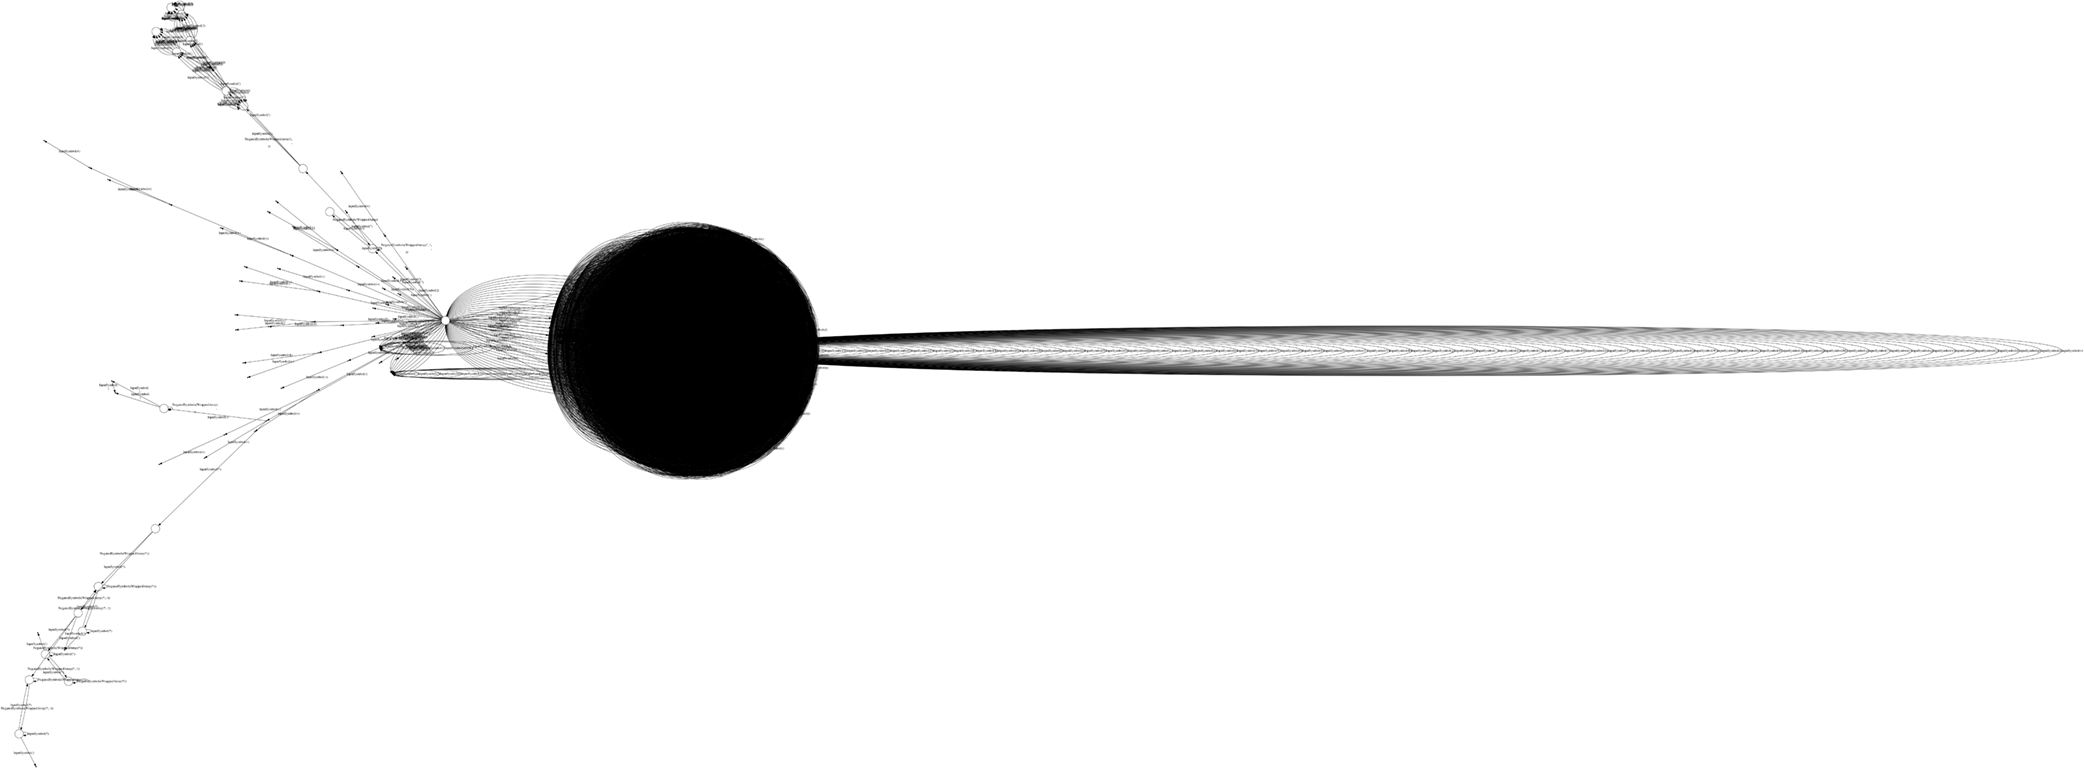
\includegraphics[width=1\textwidth]{thejoosdfa.png}
  \end{figure}

  \subsection{Parser}

  Joosbox uses an LALR(1) grammar to parse Joos1W. This grammar is based on a
  LALR(1) grammar for Java 1 itself, with numerous tokens removed and altered to
  match the language features we were supporting as specified by Joos1W. The
  LALR(1) grammar for Java 1 that we derived our grammar from was found in
  Chapter 19 of {\em The Java Language Specification}. From this collection of
  production rules for a Java 1 LALR(1) grammar, we were able to construct our
  grammar in the form of {\tt joos1w.cfg}.

  Joosbox also made use of the provided {\tt jlalr1.java} program for
  constructing a parse table from a {\tt.cfg} file. With this program we were
  able to construct a LALR(1) parse table for our grammar in the form of
  {\tt joos1w.lr1}. This file was used at runtime by Joosbox to parse the Joos1W
  language.

  To parse the sequence of tokens output by the lexer, Joosbox first discards
  tokens that do not have corresponding semantic value in the grammar (i.e.
  whitespace, comments, etc.) in a ``pre-parse weeding'' step. At this step, any
  tokens that are lexically valid but not semantically valid in Joos (including
  Java constructs that are reserved keywords, but not supported, like {\tt
  throw}) will cause a {\tt SyntaxError} to be raised.

  Once the input tokens are pre-weeded, the LR(1) algorithm with tree building
  (from CS 241) is used to construct a basic parse tree. The resulting parse
  tree output is built out of {\tt ParseTreeNode}s, arbitrary expressions that
  can contain zero or more child nodes and an optional value.

  {\tt ParseTreeNode} is implemented as an abstract class in Scala, with all of
  the different types of nodes (corresponding to symbols in the grammar) being
  concrete subclasses. These subclasses are automatically generated by a Python
  script that reads in the {\tt joos1w.lr1} file and outputs Scala classes that
  correspond to each kind of symbol in the grammar. This allows Joosbox to make
  use of Scala's strong built-in type system, adding an additional layer of
  safety to our code.

  \subsection{Abstract Syntax Tree}

  Joosbox accomplishes weeding, or post-parsing validation of semantic input, as
  a validation step during the construction of the Abstract Syntax Tree.

  A single recursive method, {\tt AbstractSyntaxNode.fromParseNode}, is
  responsible for taking a {\tt ParseNode} instance generated by the parser and
  converting it to a {\tt AbstractSyntaxNode}. {\tt AbstractSyntaxNode}s are
  desirable over {\tt ParseNode}s due to their semantic meaning --- while {\tt
  ParseNode}s represent a program, they are fairly generic and do not encode the
  semantic meaning of each node of the tree. For instance, a method declaration
  may be represented by a {\tt ParseNode} with an arbitrary number of children,
  but is more usefully represented as an {\tt AbstractSyntaxNode} with dedicated
  class members for method name, modifiers (public, static, etc), member type,
  formal parameters, and optional body. Having these parameters extracted from
  the node's syntax tree allow us to more easily implement methods that require
  information about the semantic meaning of the language constructs.

  To implement weeding during the construction of the Abstract Syntax Tree, the
  {\tt fromParseNode} method includes validations when it creates an {\tt
  AbstractSyntaxNode} from a {\tt ParseNode}. Each different type of {\tt
  AbstractSyntaxNode}  has its own validation checks --- for instance, an {\tt
  InterfaceMemberDeclaration} cannot be static  or final. When this node is
  created, its factory method ensures that this validation passes. If the
  validation  fails, a {\tt SyntaxError} is thrown indicating the type and
  source of the error.

  \section{Challenges}

  One challenge was to get our compiler to build on the Marmoset server. We used
  {\em sbt} to build, run, and test our compiler locally, but the jar files that
  were generated had third-party dependencies that would not run on the CS
  environment. We introduced the third-party library {\em sbt-assembly} to
  create a fat jar that contains our compiler and all of our third party
  dependencies, and we invoke the assembly script in our makefile to create the
  jar, and to create the executable {\tt joosc} script to invoke the jar with the
  command line arguments.

  An additional challenge when writing both the lexer and the parser for Joosbox
  was finding a way to use Scala's type system to guarantee type safety for our
  program. Each type of token in the lexer and each type of symbol in the parser
  was implemented as a separate case class in Scala, enabling us to perform
  pattern matching and extraction on tokens and parse tree nodes. To enable
  these features without writing hundreds of repetitive classes by hand, two
  small Scala code generators were written in Python.  {\tt
  lexer-type-generator.py} and {\tt parser-type-generator.py} both consume input
  files describing the types of the lexer tokens and parser tokens, and use
  these files to generate valid Scala code that implements this type hierarchy.
  These generators were tricky to write, as most code generators are, and
  required a lot of trial and error to result in correct Scala code output.
  Additionally, the huge number of Scala classes defined by the resulting
  generated code has resulted in longer compile times and larger binaries ---
  but enabled cleaner and safer code to be written.

  \section{Testing}

  For testing, we used {\em specs2}, a Scala specifications and testing library.
  We ran our tests using {\em sbt}.

  Joosbox has unit tests for small units of functionality. We individually
  tested each piece of functionality, and small portions of the lexer, parser,
  and AST generator. Our project is separated into separate sub-projects that
  deal exclusively with lexing, parsing, and code generation, and for each
  subproject, we have a separate set of specific tests.

  We used TDD (test-driven development) to develop our compiler. For each
  portion of work we started, we wrote passing and failing tests to verify the
  validity of the portion of the program we were working on.

  We imported the Marmoset tests into our local test suite, parsed each test to
  determine if they were passing or failing tests, and generated a unit test for
  each marmoset test. This substantially increased our development speed, as
  this integrated our regular unit testing strategy with the Marmoset tests, and
  also avoided needing to upload a zip file to Marmoset after every code
  iteration.

\end{document}
